%-*- coding: UTF-8 -*-
% 论文总结.tex
% 2020年7月第四周
\documentclass[UTF8]{ctexart}
\usepackage{graphicx}
\usepackage{float}
\usepackage{amsmath}
\usepackage{geometry}
\geometry{a4paper,centering,scale=0.8}
\usepackage[format=hang,font=small,textfont=it]{caption}
\usepackage[nottoc]{tocbibind}
\usepackage{url}
\usepackage{listings}
\usepackage{booktabs}
\usepackage{xcolor}     %高亮使用的颜色
\definecolor{commentcolor}{RGB}{85,139,78}
\definecolor{stringcolor}{RGB}{206,145,108}
\definecolor{keywordcolor}{RGB}{34,34,250}
\definecolor{backcolor}{RGB}{220,220,220}

\lstset{
 columns=fixed,       
 numbers=left,                                        % 在左侧显示行号
 numberstyle=\tiny\color{gray},                       % 设定行号格式
 frame=none,                                          % 不显示背景边框
 backgroundcolor=\color[RGB]{245,245,244},            % 设定背景颜色
 keywordstyle=\color[RGB]{40,40,255},                 % 设定关键字颜色
 numberstyle=\footnotesize\color{darkgray},           
 commentstyle=\it\color[RGB]{0,96,96},                % 设置代码注释的格式
 stringstyle=\rmfamily\slshape\color[RGB]{128,0,0},   % 设置字符串格式
 showstringspaces=false,                              % 不显示字符串中的空格
 language=c++,                                        % 设置语言
}

\newenvironment{myquote}
{\begin{quote}\kaishu\zihao{-5}}
{\end{quote}}

\newcommand\degree{^\circ}

\title{\heiti Deep Neural Networks for YouTube Recommendations }
\author{\kaishu 宇翔}
\date{\today}

\bibliographystyle{plain}

\newtheorem{thm}{定理}

\begin{document}
    \section{摘要}\label{sec:diyijie}
    本文介绍了深度学习在YouTube的推荐系统中的应用,详细说明了深度候选模型(deep candidate generation model)以及深度排序模型(separate deep ranking model)。

    YouTube推荐系统面临的三大挑战:
	\begin{itemize}
		\item[·] Scale视频、用户量大
		\item[·] Freshness:The recommendation system should be responsive enough to model newly uploaded content as well as the latest actions taken by the user. 推荐系统需要能够对新上传的视频和最新的用户行为进行快速建模,作出推荐,并平衡新老视频的综合推荐。
		\item[·] Noise:Historical user behavior on YouTube is inher- ently difficult to predict due to sparsity and a vari- ety of unobservable external factors. We rarely obtain the ground truth of user satisfaction and instead model noisy implicit feedback signals.由于稀疏性及不可观察的外部特性,用户行为很难被预测;推荐系统需要对隐式的反馈信号(对应的是显式的用户满意度反馈,但通常这种反馈很少)进行建模。推荐算法必须对数据有足够的鲁棒性。
	\end{itemize}
	
	该系统基于TensorFlow搭建在Google Brain上,推荐模型的参数有10亿之多,并经过了超千亿的样本训练。
    \clearpage

	\section{系统概述}\label{sec:dierjie}
	推荐系统的总体结构如图1所示,该系统有两个神经网络组成:候选阶段(搜索/召回)和排序阶段。
	\begin{figure}[ht]
        \centering
        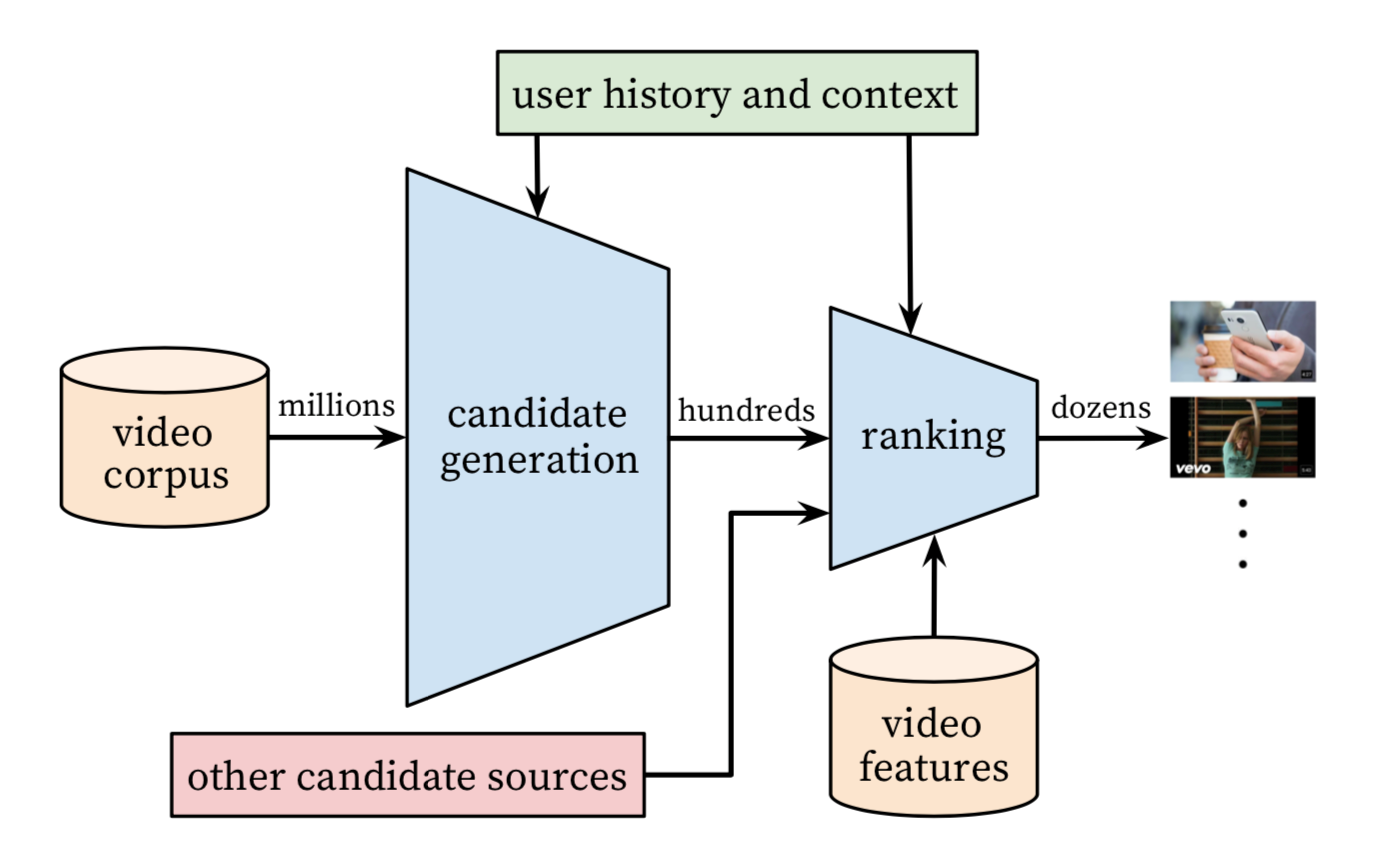
\includegraphics[scale=0.5]{picture/001.png}
        \caption{框架}
        \label{fig:001}
    \end{figure}
    \begin{itemize}
		\item[·] 候选:用户的历史行为作为输入,从大量数据集中检索出部分(上百)与用户高度相关的子集,此部分可以通过协同过滤、粗糙的特征(如观看过的视频,搜索记录,用户画像等)进行检索;
		\item[·] 排序:利用上述候选模块筛选出来的候选集,结合更丰富的特征,对每个候选进行打分排序,依据得分从高到底进行推荐。
		\item[·] 评价指标:线下评价(precision,recall,ranking loss); 线上评价(A/B test,点击率、观看时间)
	\end{itemize}
	\clearpage

	\section{深度候选模型}\label{sec:disanjie}

    \begin{itemize}
		\item[·] 候选模型目的:在大量Youtube视频中检索出数百个和用户相关的视频作为候选。
		\item[·] 作者将推荐任务转化为一个多分类问题,把每一个视频当作一个分类,则给定用户U和上下文C的条件下,在时间t观看第i个video(第i类)的概率为:
		\begin{equation}\label{eq:gongshi1}
			\begin{aligned}
		    	&P(\omega_t=i|U,C)=\frac{e^{v_iu}}{\sum_{j\in V}e^{v_ju}}\qquad)
    		\end{aligned}
    	\end{equation}
    	其中u是用户的向量表示(embedding),v是video的向量表示(embedding)。在模型中,利用用户历史和上下文来学习用户的embedding,利用用户的embedding对每个用户进行视频推荐;类似于Word2vec,模型在训练过程中可以利用负采样进行优化。
    	\item[·] 在深度候选模型中,DNN的任务是基于用户的历史及场景,学习一个用户向量u的映射函数(embedding),通过一个softmax分类器,u能够有效的从视频语料库中识别视频的类别(也就是推荐的结果)。模型架构如下图所示:
		\begin{figure}[ht]
	        \centering
	        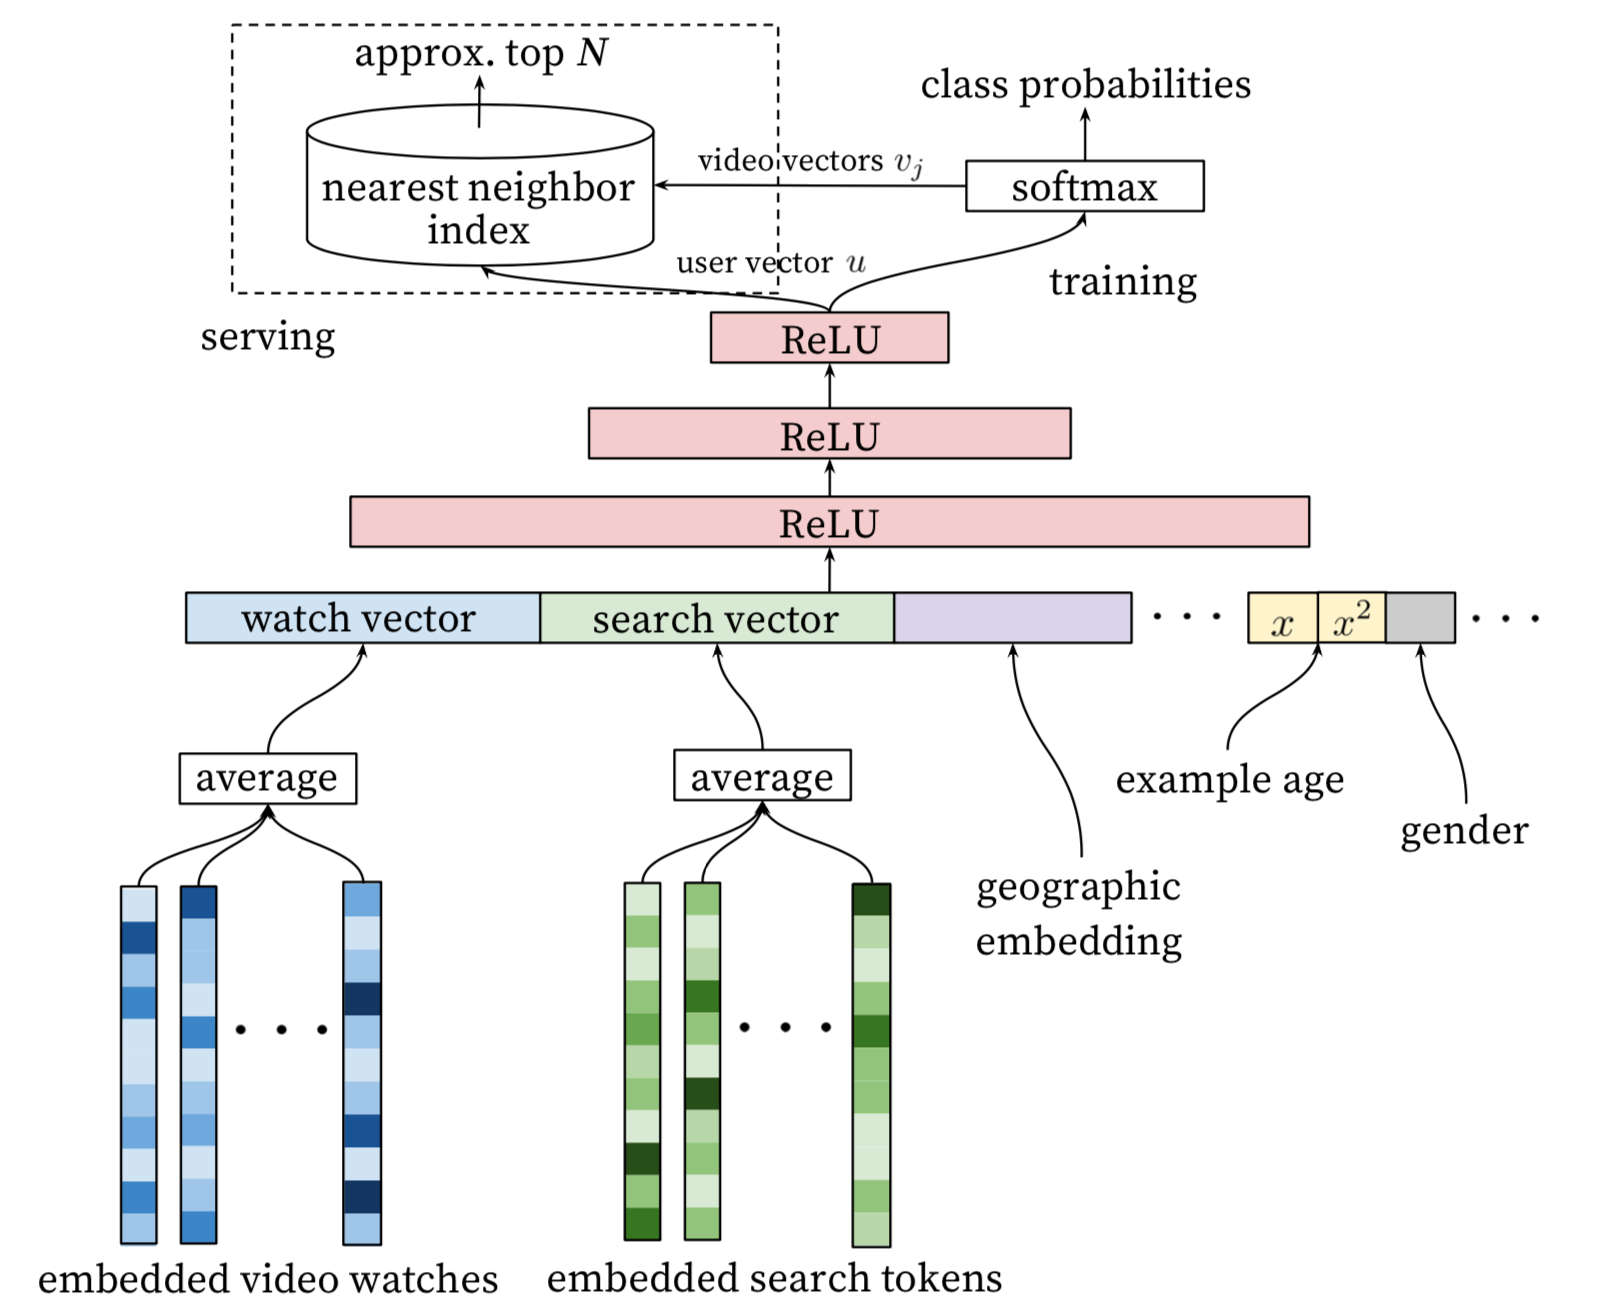
\includegraphics[scale=0.5]{picture/002.png}
	        \caption{深度候选模型}
	        \label{fig:002}
	    \end{figure}
		\end{itemize}
		模型输入:用户历史观看embedding,历史搜索embedding,画像特征,年龄、性别等

		模型输出:用户观看每个视频的概率,topn推荐

		模型中,首先获取各个特征进行拼接,作为网络的输入,经过一系列隐藏层得到用户embedding,根据用户embedding与video embedding即可计算该用户在时间t观看视频的概率,依据概率分布选取top N作为候选推荐子集。
	\clearpage
	\section{针对深度候选模型的几个关注点}\label{sec:disijie}
	\subsection{主要特征的处理}
	列表内容观看和搜索向量的生成: 用户的历史观看是一个稀疏的,变长的视频id序列,作者对每一个视频从固定的词汇表里计算出一个多维词向量,这样用户的观看历史就可以通过加权平均的方式映射为一个稠密的,定长的watch vector。整个过程类似于word2vec算法。Search vector也可以通过类似的方式生成。

	用户画像特征:如地理位置,设备,性别,年龄,登录状态等连续或离散特征都被归一化为[0,1], 和watch vector以及search vector做拼接。
	
	example age:该特征表示视频被上传之后的时间。YouTube每秒钟都有大量视频被上传,推荐这些最新视频对于YouTube来说是极其重要的。作者持续的观察到,用户更倾向于推荐那些尽管相关度不高但是是最新(fresh)的视频。推荐系统往往是利用用户过去的行为来预测未来,那么对于历史行为,推荐系统通常是能够学习到一种隐式的基准的。但是对于视频的流行度分布,往往是高度不稳定的。作者写道,在之前的处理上,训练所选择的时间窗口,是采用最近几周的用户平均观看似然率来进行推荐的。那么考虑到example age的现象,我们的推荐策略将example age作为一个特征拼接到DNN的输入向量。训练时,时间窗口越靠后,该值越接近于0或者为一个小负数。加入了example age特征后,模型效果和观测到的实际数据更加逼近(如图3)。
	\begin{figure}[ht]
	    \centering
	    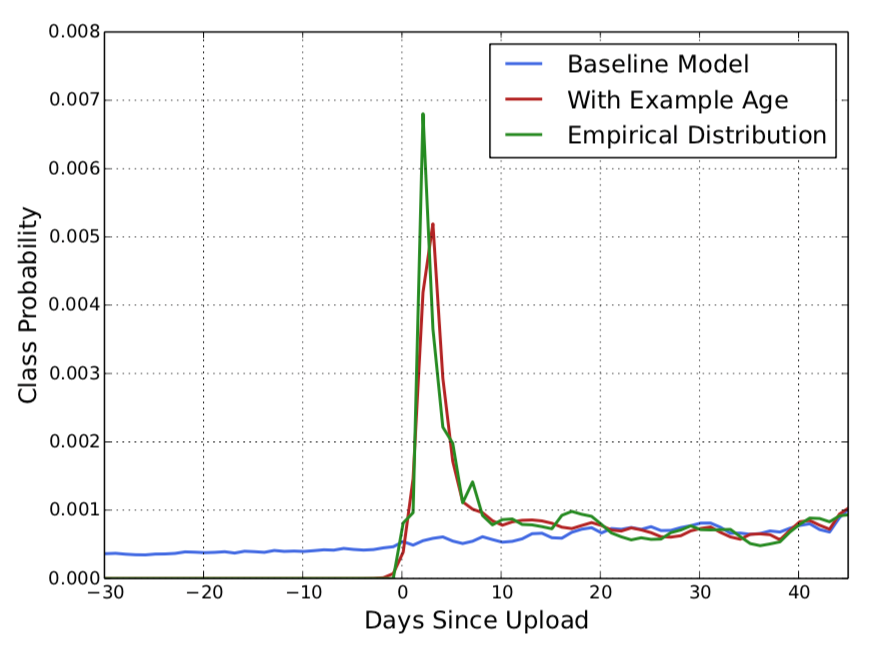
\includegraphics[scale=0.5]{picture/003.png}
	    \caption{训练数据集}
	    \label{fig:003}
	\end{figure}
	\subsection{标签和上下文选择}
	样本来源:训练样本来源于全部的YouTube观看记录,而不仅仅是被推荐的观看记录,否则对于新视频会难以被曝光,会使最终推荐结果有偏;同时系统也会采集用户从其他渠道观看的视频,从而可以快速应用到协同过滤中;

	样本数量:每一个用户都会有固定数量的训练样本,在损失函数中的权重是相同的,这样可以防止那些活跃用户对模型的影响。

	序列无序化:如果每次推荐都仅仅是和最后一次搜索相关,推荐结果会是糟糕的,所以为了防止过拟合,将序列无序化,分类器不会再直接获取序列的原始值,效果会更加鲁棒。

	训练数据选择:用户观看视频时,遵循的是一种非对称的观看模式,在初始的观看序列中,范围会比较广泛,在后期的观看中,范围会逐渐集中。而大部分协同过滤算法,在推荐时往往利用的是用户的全量观看历史。所以,作者的改进在于从用户的观看历史序列中,只截取held-out watch之前的观看序列。该过程可以描述如图4.
	\begin{figure}[ht]
	    \centering
	    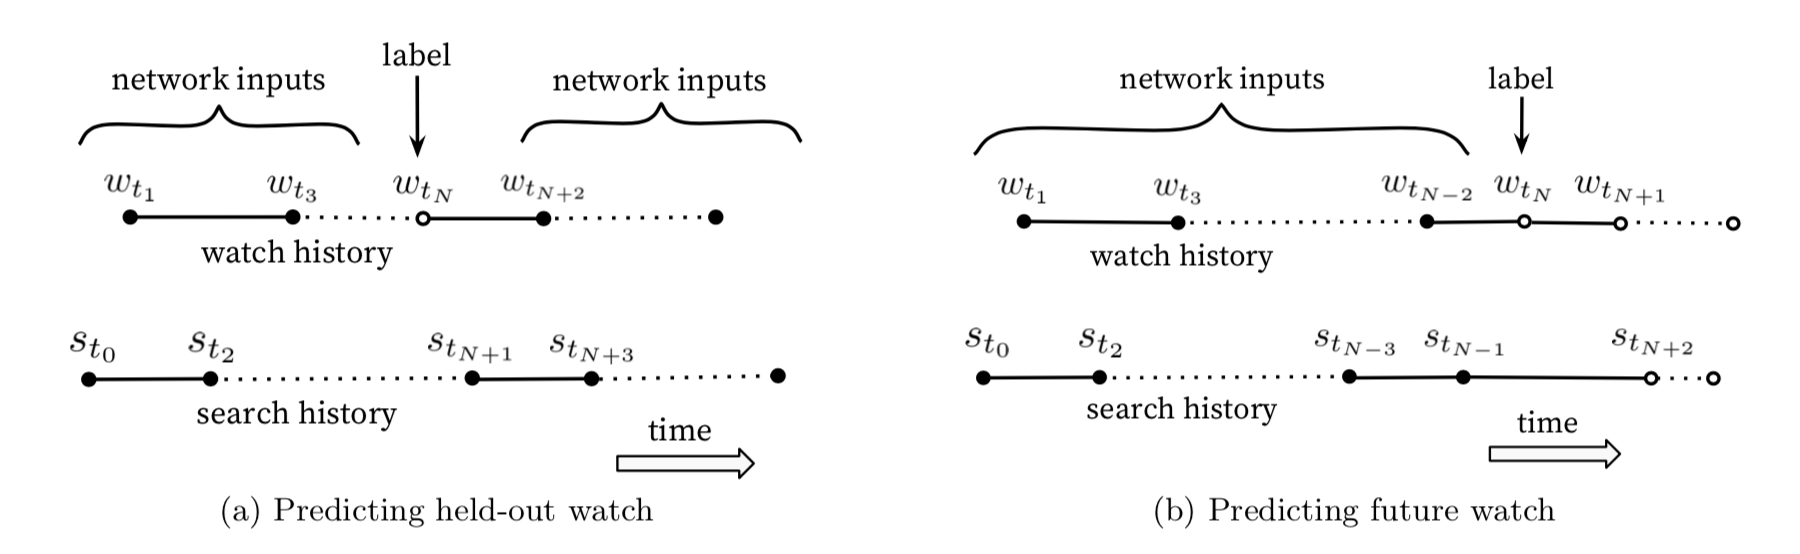
\includegraphics[scale=0.5]{picture/004.png}
	    \caption{example age}
	    \label{fig:004}
	\end{figure}
	图4中,(a)是许多协同过滤会采取的方法,利用全局的观看信息作为输入(包括时间节点N前,N后的观看),这种方法忽略了观看序列的不对称性,而本文中采取(b)所示的方法,只把历史信息当作输入,用历史来预测未来。

	\subsection{特征集以及深度的实验}
	添加特征以及DNN深度可以显著提升预测效果,但并非一直如此。第0层的输入向量全连接到softmax输出层,第0层以及输出层都是采用固定的256维度。中间的深度网络采用的是类似tower的结构。深度增加时,预测效果如下图.
	\begin{figure}[ht]
	    \centering
	    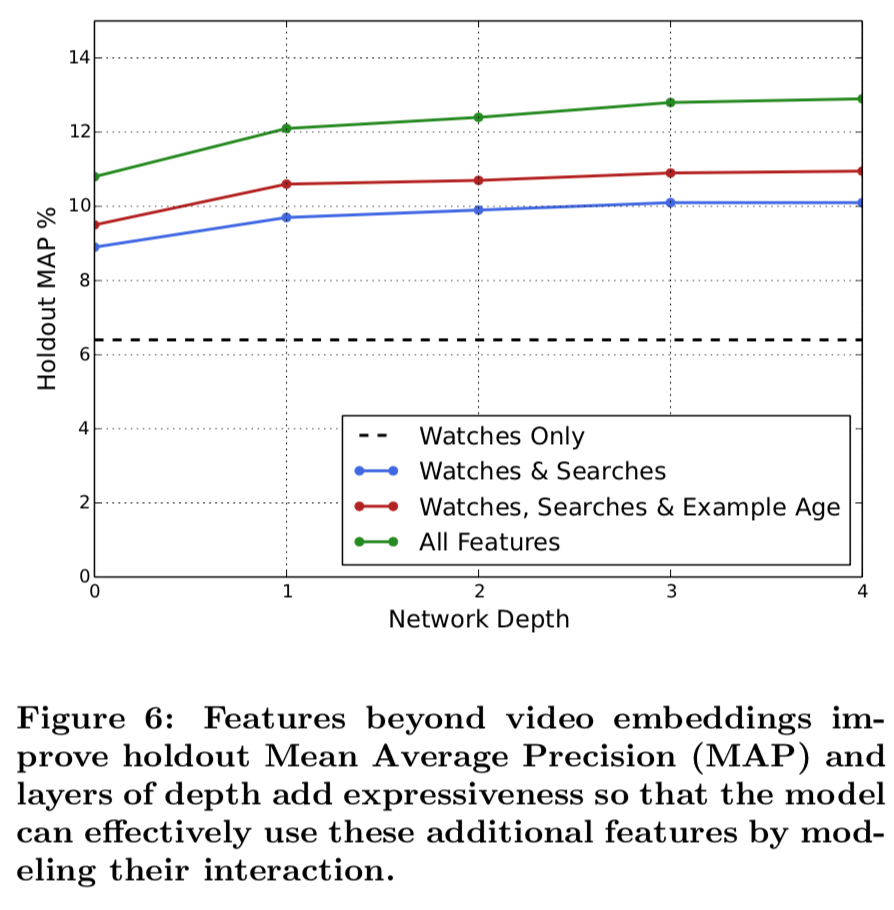
\includegraphics[scale=0.5]{picture/005.png}
	    \caption{DNN}
	    \label{fig:005}
	\end{figure}
	由图中可以看出,添加特征和模型深度可以使模型表现更好,但是当层数增加到4时,效果提升并不明显。
	\section{深度排序模型}\label{sec:diwujie}
	深度排序模型目的:对深度候选模型输出得到的候选序列再次进行建模,为每个推荐进行打分,按照得分排序进行推荐。
	排序模型架构:
	\begin{itemize}
		\item[·] 模型输入:video embedding,language embedding,上次观看时间等一系列特征
		\item[·] 模型输出:利用逻辑回归进行打分,返回各个推荐的得分(根据得到的点击概率进行排名)
		\item[·] 目标变量:期望观看时间
	\end{itemize}
		\begin{figure}[ht]
	    \centering
	    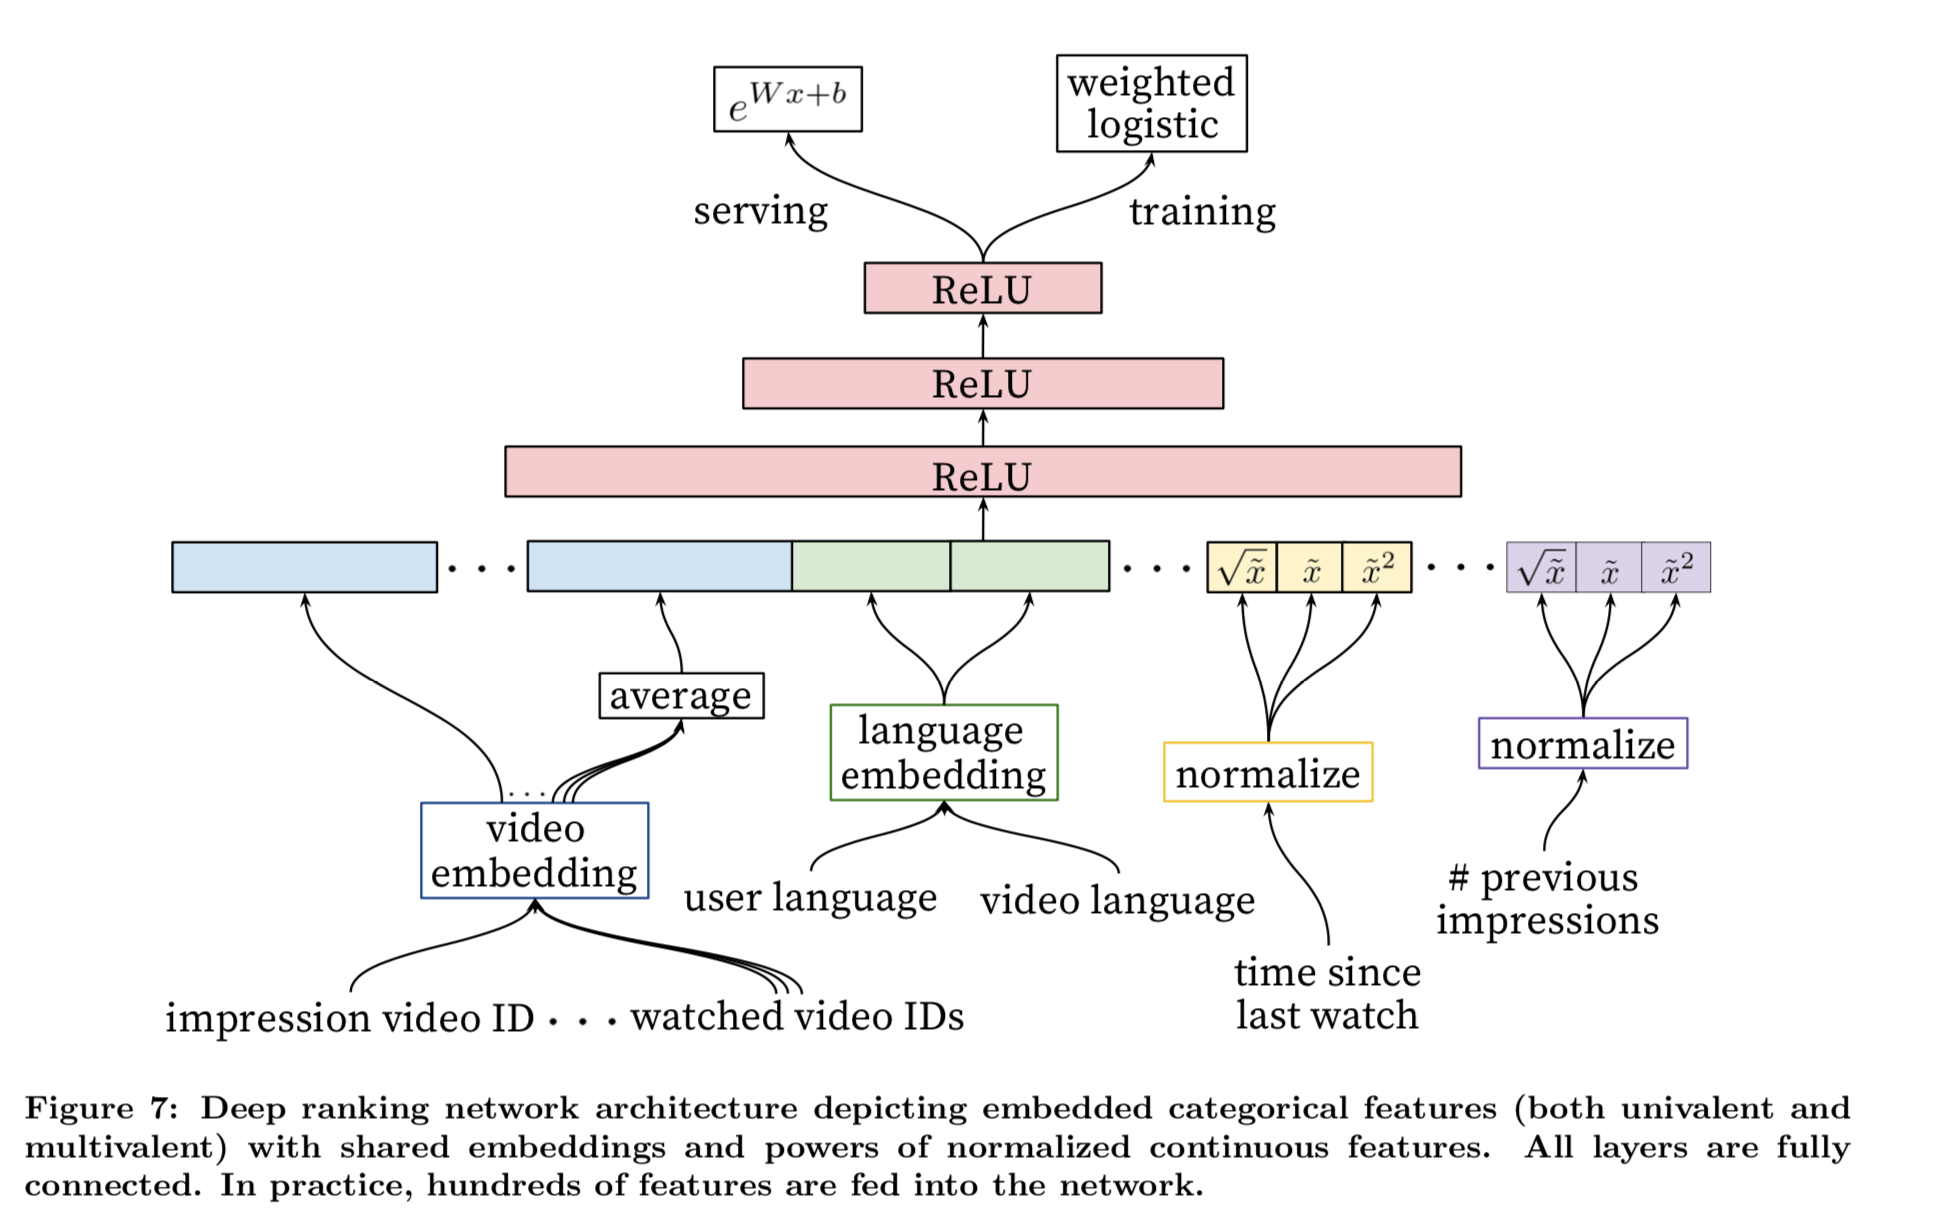
\includegraphics[scale=0.5]{picture/006.png}
	    \caption{深度排序模型}
	    \label{fig:006}
	\end{figure}
	\clearpage
	\section{针对深度排序模型几个关注点}\label{sec:diliujie}
	模型特征:尽管神经网络能够减轻人工特征工程的负担,但是作者依然花费精力将用户及视频数据转化为有效的特征。而其难点在于对用户行为序列建模,并关联视频打分机制。如:用户从这个频道观看的video个数;用户最后一次浏览该话题的时间;推荐的来源;推荐来源的得分;是否推荐过但是没看;用户是否登录;用户看的最后N个视频embedding;用户上次搜索序列embedding;用户特征、商品特征等。
	
	类别特征embedding:作者依然采用embedding的方式映射稀疏离散特征为密集向量,作者为每一个类别特征维度生成一个独立的embedding空间。值得注意的是,对于相同域的特征可以共享embedding,其优势在于加速迭代,降低内存开销。
	
	连续特征归一化:NN对于输入的分布及特征的尺度敏感。作者设计一种积分函数将特征映射为一个服从[0,1]分布的变量。该积分函数为: $\tilde{x} = \int_{-\infty}^{x}df $.

	对观看时间建模:划分样本空间时,正样本为有点击视频,负样本为无点击视频,作者采用一种加权逻辑回归基于交叉熵损失进行训练。加权方案为,正样本用观看时间赋予权值,负样本赋予单位权值。在这种方案下,逻辑回归几率为: $\frac{\sum T_i}{N-k} $.并根据该几率,能够推导出可以采用自然指数作为预测节点的激活函数。

	隐层数的实验与召回阶段DNN的方法类似。
	\clearpage
	\section{个人笔记}\label{sec:diqijie}
	本文先总体介绍了视频推荐系统的整体架构,之后分成候选集生车及排序两个阶段分别阐述模型架构,训练数据选择、特征处理以及训练过程及训练结果。尤其是在训练数据选择和特征处理时,需要准确分析实际场景和需求。

	但是由于对深度学习、分类问题知识还不够完善,阅读本文只是对如何阐述针对一个具体问题的机器学习模型有了大致的认识,但是具体的分析部分还是有很多不理解,在工程应用方面的指导也没有get到其中的精华。该论文作为推荐系统领域的经典论文,后续完善相关知识后,可以重读。
	\clearpage
	\section{相关知识}\label{sec:diqijie}
	
	深度学习:http://www.woshipm.com/ai/2585485.html(比较浅显点)

	Embedding:Embedding是一种典型的利用无监督信息提升监督问题解决效果的手段。https://zhuanlan.zhihu.com/p/53058456
	\clearpage
	\bibliography{test}
\end{document}

